\chapter{Design}~\label{cha:design}
Before initiating detailed design work, it was decided this project would be a web application accessible via a browser. This approach offers several advantages, such as cross-platform compatibility, ease of access (requiring only a browser), scalability, and the ability to leverage existing web technologies~\cite{6822300}. With this established, a plan was formulated, including selecting the architectural model and technology stack. Testing criteria were also defined during this stage.

\section{Architecture}
The system architecture defines the overall structure of the project and the communication between its components. For this project, two architectural approaches were considered: a monolithic architecture and a microservices-based architecture.

\subsection{Monolithic}
In a monolithic architecture, all components of the application are combined into a single program, with all code running in a single process~\cite{10.1145/3241403.3241440}. This would have offered several benefits. With all code centralised within a single framework, development is simplified, and debugging becomes more straightforward~\cite{sym14091824}. Additionally, initial deployment is less complex since only one program needs to be managed~\cite{9109514}. Many examples exist of a monolithic design in web applications such as Instagram, which, as of $2025$, is a monolith written in Python~\cite{InstagramMonolith}.

However, the monolithic design has its drawbacks. Maintaining a large, integrated codebase can become increasingly challenging as the system grows. For example, test suites may grow more complex and time-consuming to execute, or during deployment, a single fault could bring down the entire system, resulting in a complete loss of service. Similarly, even minor updates would require redeploying the whole monolith, increasing downtime. Moreover, this approach does not scale as effectively for web applications; as user demand increases, the need to redeploy the monolith frequently to manage higher request volumes becomes a significant concern~\cite{9109514}.

Although the drawbacks of a monolithic approach would have minimal impact on a project of this size, it was decided to build the project in a manner that should be as scalable as possible. If the project were to grow in terms of features and users, the limitations inherent in a monolithic architecture could eventually become a hindrance. Consequently, the monolithic approach was ruled out in favour of a more scalable architectural model, though it should be noted that a monolithic design is not inherently unscalable.

\begin{figure} [H]
    \centering
    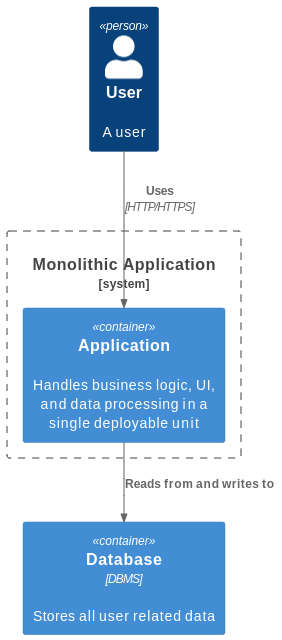
\includegraphics[width=0.35\linewidth]{figures/monolithic_arch.png}
    \caption{A potential architecture for a monolithic approach}
~\label{fig:monolith-arch}
\end{figure}

\subsection{Microservices}
The alternative approach examined was the use of microservices. In this architecture, the application's functionality is split into many small services that communicate with each other using standardised protocols such as HTTP~\cite{8354423}. This approach is used widely in modern web development, with one example being Netflix~\cite{NetflixMicroservices}. Notably, the services themselves do not need to be implemented in the same language~\cite{7030212} as long as the interface between them is standardised.

The primary benefits of this approach pertain to deployment and maintenance. Once deployed, the system can be scaled more efficiently. Only those services experiencing high demand need to be replicated, which is significantly faster and more resource-efficient than scaling a monolithic system~\cite{9717259}. Additionally, maintenance is simplified because each service operates independently. A comprehensive understanding of all other services is not required to work on any individual service. In this project, this is not a significant issue but in large code bases, this can be advantageous.

However, the increased complexity of managing multiple services makes the initial deployment more challenging~\cite{9717259}. Configuring the different addresses for inter-service communication can prove to be tedious, and each service requires setup that would only need to be completed once for a monolith. Once this initial configuration is completed, development within a microservice architecture becomes as straightforward as working with a monolithic architecture.

\begin{figure} [H]
    \centering
    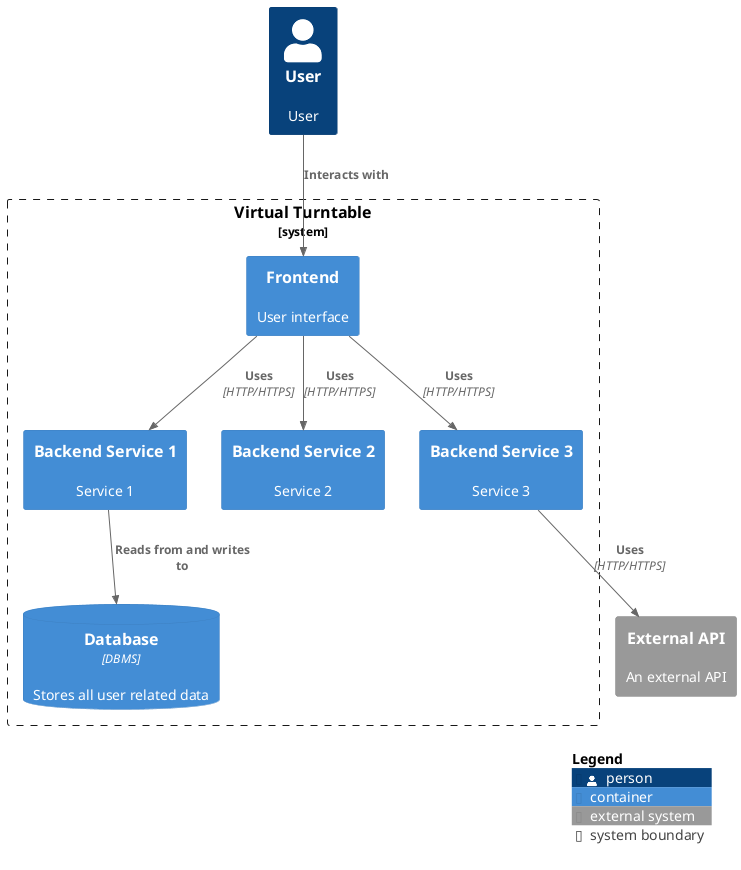
\includegraphics[width=0.4\linewidth]{figures/microservices_arch.png}
    \caption{A potential microservices design with three backend services}
    \label{fig:microservices-arch}
\end{figure}

\subsection{Final design}
The final design employs a microservices approach alongside a backend-for-frontend (BFF) design pattern. In this pattern, a dedicated backend service, the BFF, is created for each type of frontend application, such as desktop or mobile, ensuring that each backend caters to a specific interface’s requirements. This pattern leverages the benefits of a microservices architecture and helps reduce complexity by isolating functionality particular to a single frontend~\cite{BFF}. There are also security benefits as users need only to authenticate with a single service rather than each of the microservices individually. Details about each microservice are described in Section~\ref{sec:backend-design}.

\begin{figure} [H]
    \centering
    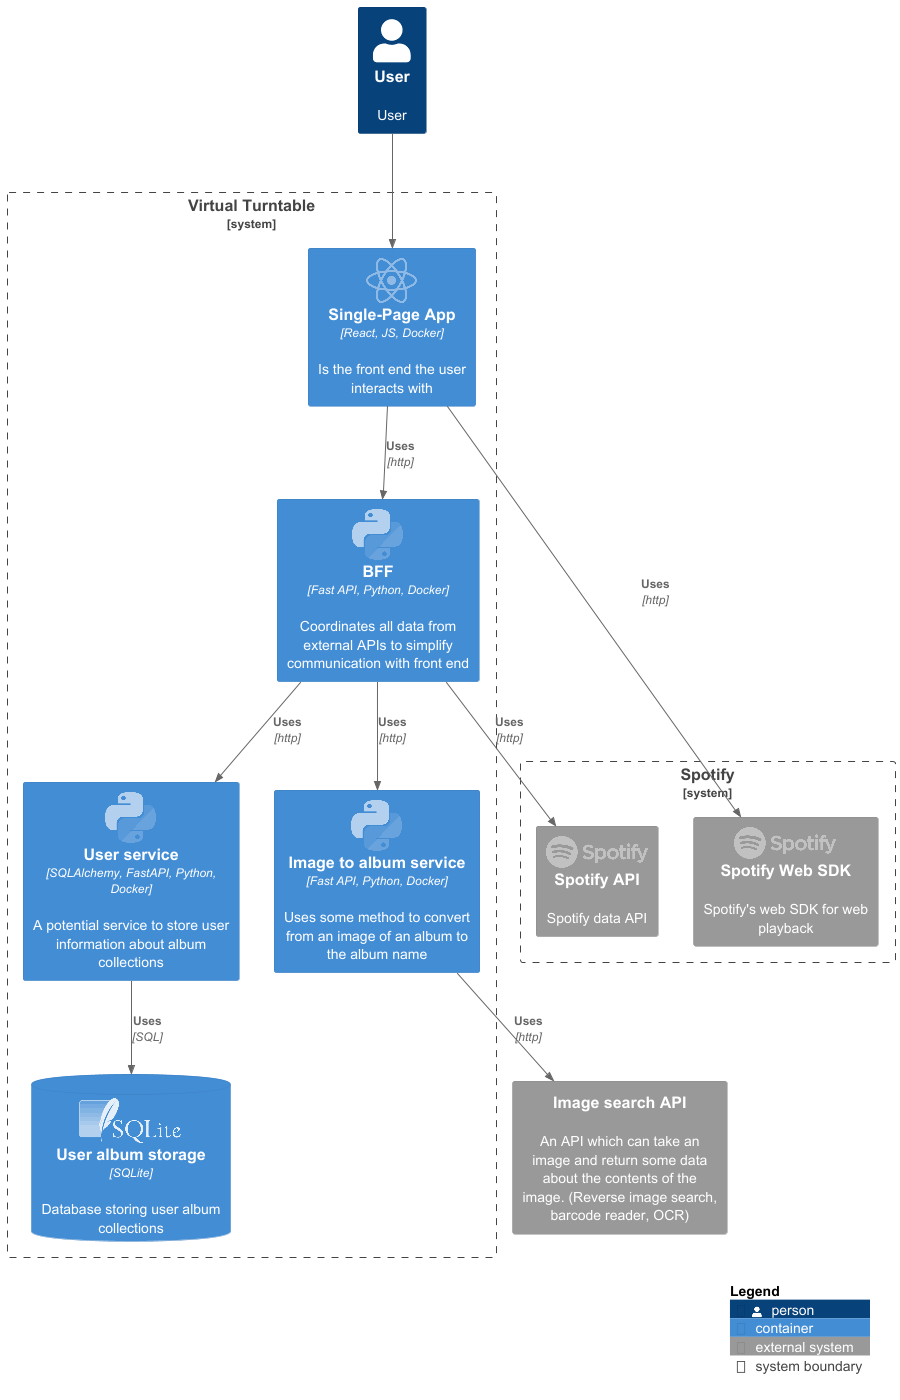
\includegraphics[width=0.5\linewidth]{figures/final_arch.png}
    \caption{The final architecture including technologies and external APIs}
    \label{fig:final-arch}
\end{figure}


\section{Technologies}
\subsection{FastAPI}
FastAPI is a Python web framework for building APIs; it provides automatic input validation via Pydantic and easy-to-use relational database integration with SQLAlchemy \cite{FastAPI}. Its native support for these provided much of the boilerplate functionality required for the project, reducing development time. Compared to other popular frameworks like Django and Flask, FastAPI was particularly well-suited for this project due to its lightweight nature, which is essential for a microservice approach~\cite{9717259}.

All backend services were to be implemented using FastAPI extensively. Its straightforward setup allowed for rapid initial setup and development, and its flexibility enabled the implementation of more complex features as development progressed.

The backend primarily operated through individual API endpoints, which the frontend called to retrieve data as needed. Additionally, WebSockets facilitated asynchronous server-to-client communication, allowing users to be notified of backend events, such as collections being shared with them.

\subsection{React}
React is a JavaScript library for building interactive web interfaces~\cite{React}. Its modular, component-based architecture was particularly beneficial in this project, enabling component reuse and reducing code duplication~\cite{10638895}. A key advantage of this approach is the availability of extensive component libraries that provide pre-built functionality and styling for low-level elements, such as buttons, allowing development efforts to focus on the application's bespoke features.

For this project, the HeroUI component library was utilised~\cite{HeroUI}. It offered a set of pre-designed components that could be assembled into larger, more complex bespoke UI elements to create the final application.

React also managed the application's state and handled backend requests as needed. This choice allowed backend services to remain stateless, reducing complexity and improving scalability.

An alternative approach using plain JavaScript and HTML was considered as for a smaller project the initial setup would be much faster but the lack of scalability and maintainability would have been a significant issue as the project grew. Testability would also have been a problem as it would be difficult to test parts of the application in isolation.

\subsection{Docker}
The application had many dependencies which had to be installed to run the application correctly. This presents a challenge of how to ensure the correct versions are installed at build or run time. A possible solution could be to just installing all required packages on the whole system, however, what if different services require different versions of the same package? A better solution would be to keep all services separate and to run them in different environments. To achieve this, Docker was used.

Docker is a platform for containerising applications, allowing them to run in isolated environments while communicating through specified exposed ports~\cite{DockerDocs}. This approach is widely supported by cloud providers~\cite{AWSDocker,GoogleDocker}, simplifying deployment and providing a consistent environment across different platforms.

For this project, Docker enabled efficient and error-free deployment. When triggered, cloud providers could autonomously build and run each of the four containers when supplied with the codebase and Dockerfile. In addition, if a user wanted to run the application locally, the containerised system could be easily launched on any device running Docker, eliminating the need for manual environment configuration.

\subsection{Spotify API And Web Playback}
The music service Spotify offers a suite of APIs for music-related services, including search and playback functionalities that matched the core features of this project~\cite{SpotifyAPI}. Given the impracticality of maintaining an independent album database, offloading the responsibility of maintaining a library of albums and music to Spotify was a logical choice.

Specifically, the search API was used to identify albums, while the playback API enabled in browser playback of the desired music.

However, a key limitation of this approach is that the playback API requires a Spotify Premium subscription~\cite{SpotifyPlaybackSDK}. However, as the Spotify API forces user authentication via a Spotify account, this requirement can be leveraged to use the user's Spotify account as a user account for the application, reducing potential security concerns about the storage and management of user data.

\subsection{Reverse Image Search}~\label{sec:reverse-image-search}
Reverse image search is a form of content-based image retrieval that uses an image to query related results. This process involves extracting feature vectors, using algorithms such as SIFT, and comparing these against a collection of previously indexed images to return the closest matches~\cite{Gaillard2017LargeSR}.

In this project, reverse image search functionality was implemented to identify albums from images uploaded by users. Recognising that maintaining an up-to-date, in-house database of album covers would be impractical, it was decided early on to leverage an external API. Two reverse image search APIs were evaluated: Google and Bing. Although Bing's API was simpler to integrate, it frequently failed to accurately identify albums, even from images already indexed by Bing's image search. In contrast, Google's API demonstrated a much higher reliability in album identification. Given the critical importance of accurate album retrieval for the project, the Google API was ultimately chosen.

Compared to other methods for recognising albums from images, such as optical character recognition (OCR) or barcode scanning, reverse image search was selected for its robustness. OCR can be unreliable when album covers feature stylised text or lack text entirely, and barcode scanning, though dependable, requires a barcode to be present. This requirement is problematic, particularly since some vinyl records may predate the widespread use of barcodes.

\subsection{Google Cloud}
Google Cloud is a suite of cloud services offered on a pay-as-you-use basis~\cite{GCP}. This project utilised two specific services: the reverse image search API and Google Cloud Run. The reverse image search API was employed to identify albums from images uploaded by users, as detailed in Section~\ref{sec:reverse-image-search}. Google Cloud Run was used to build and host the application in Docker containers.

Although multiple cloud providers were available, Google Cloud was selected following the adoption of Google's reverse image search API. For convenience, hosting the application on Google Cloud was more straightforward as it eliminated the need to manage services across different providers.

\section{Frontend}
The front end is the application's user-facing part. Because of this, it needed to be designed with the knowledge that users have a wide range of abilities and needs.

A `multipage' design approach was selected for the application as this separates the application into sections, so the user is not overloaded on a single page. Two implementation approaches were considered: a router design where the separate pages are loaded as the user navigates the application or a single page app where the screens are different `tabs'. The former would have been simpler as there would be little implementation to link the pages together. Still, it was decided to implement the latter as it would provide a more fluid user experience where the user could easily switch between different views. There was also the added benefit of allowing music playback to continue even as the user navigates the application.

\subsection{Wireframe mockups}
Prototyping the user interface provides a rapid way to visualise the application, enabling design evaluations without writing any code~\cite{WILSON1988859}. This approach proves especially beneficial during the early stages of development. At that point, designs must remain flexible so they can be easily modified as feedback is collected. In this project, wireframe mockups were selected as their low-fidelity nature allowed for fast iteration on design.

Across all mockups, a consistent navigation bar is at the top of the screen, allowing for straightforward navigation among the application's various pages.

\subsubsection{Play Screen}
Figure~\ref{fig:play_screen_mockup} depicts the mockup of the play screen, where users control music playback. Essential functionality implemented here includes buttons to play, pause, skip forward or backwards, adjust the track position, and manage volume. As the look of the controls fits what is found on popular music streaming services, users likely have experience controlling playback in this manner.

The track list displayed on the left side allows the user to select a single track from the album to play. Features like this are not found on physical turntables, but users listening online may expect functionality like this, so it was included.

The spinning vinyl in the centre of the screen had no functional purpose but was included to maintain the theme of vinyl records. For this purpose, animations also show a vinyl record being removed from a sleeve whenever the album changes.
\begin{figure} [H]
    \centering
    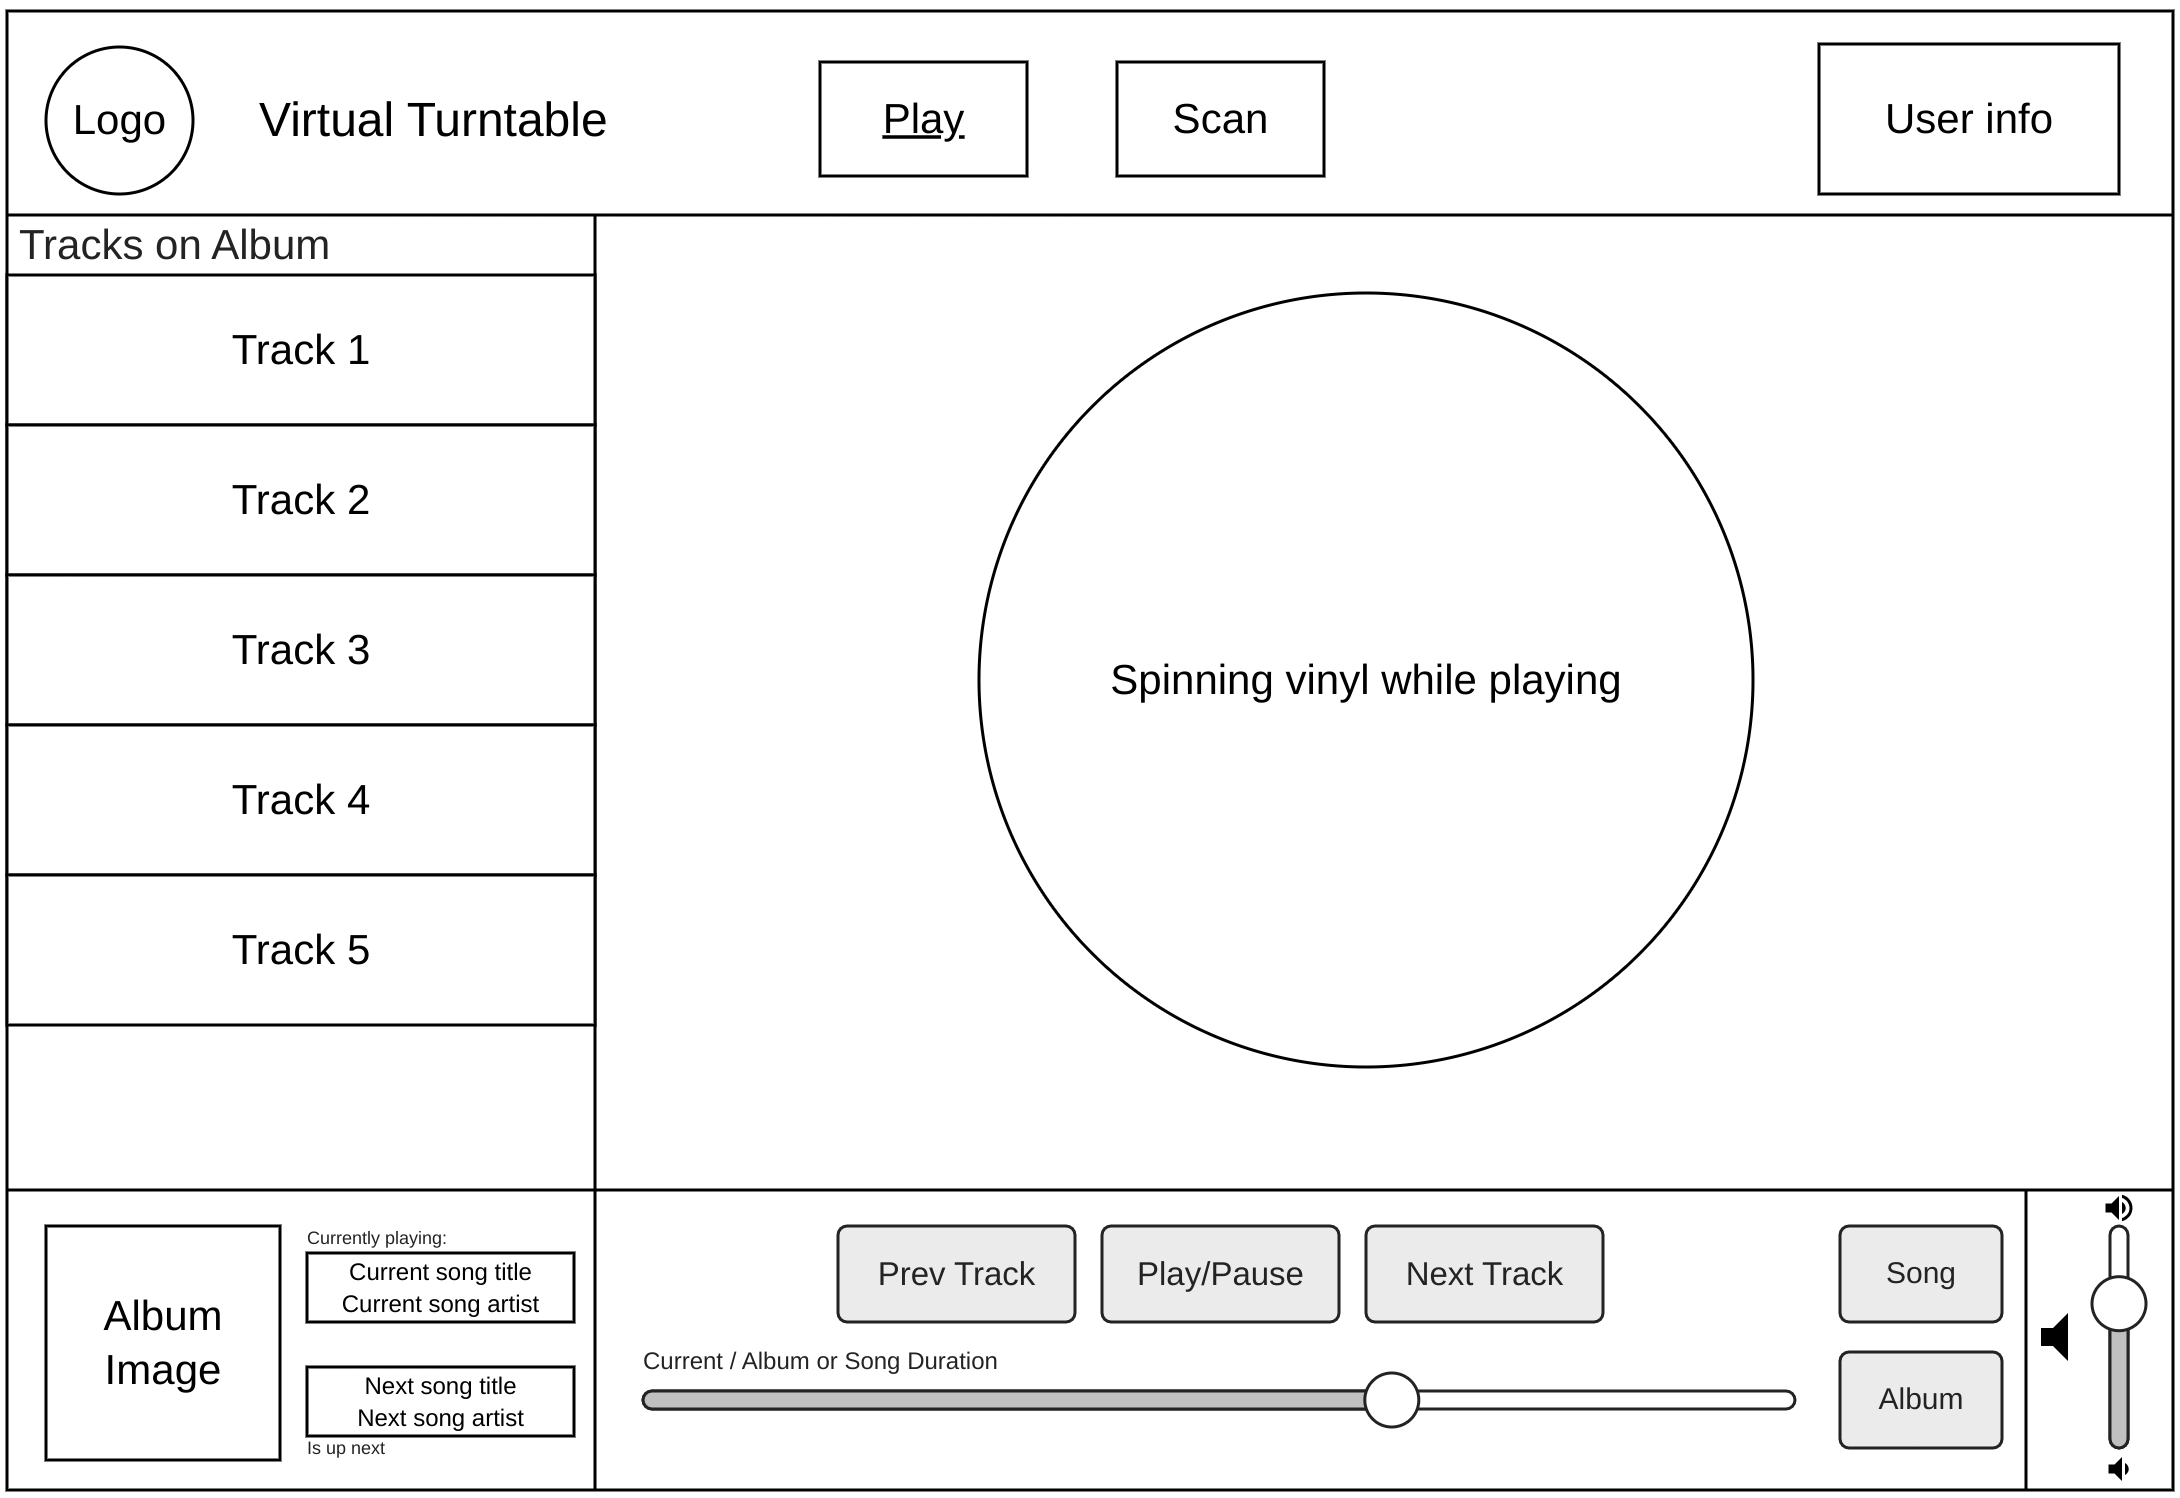
\includegraphics[width=0.6\linewidth]{figures/play_screen_mockup.png}
    \caption{The play screen wireframe mockup}
    \label{fig:play_screen_mockup}
\end{figure}

\subsubsection{Scanning Screen}
Figure~\ref{fig:scan_screen_mockup} shows the scanning screen. Here, users can take and upload images of album covers to identify the corresponding album.
At the bottom of the screen, the logged-in user’s existing album collection is displayed. This allows a quick selection of albums already scanned, meaning users only have to scan an album once.
The confirmation dialogue (shown on the left) appears after the application returns a scan result for an album. It enables users to confirm that the identified album is correct or reject it if it is incorrect.

\begin{figure} [H]
    \centering
    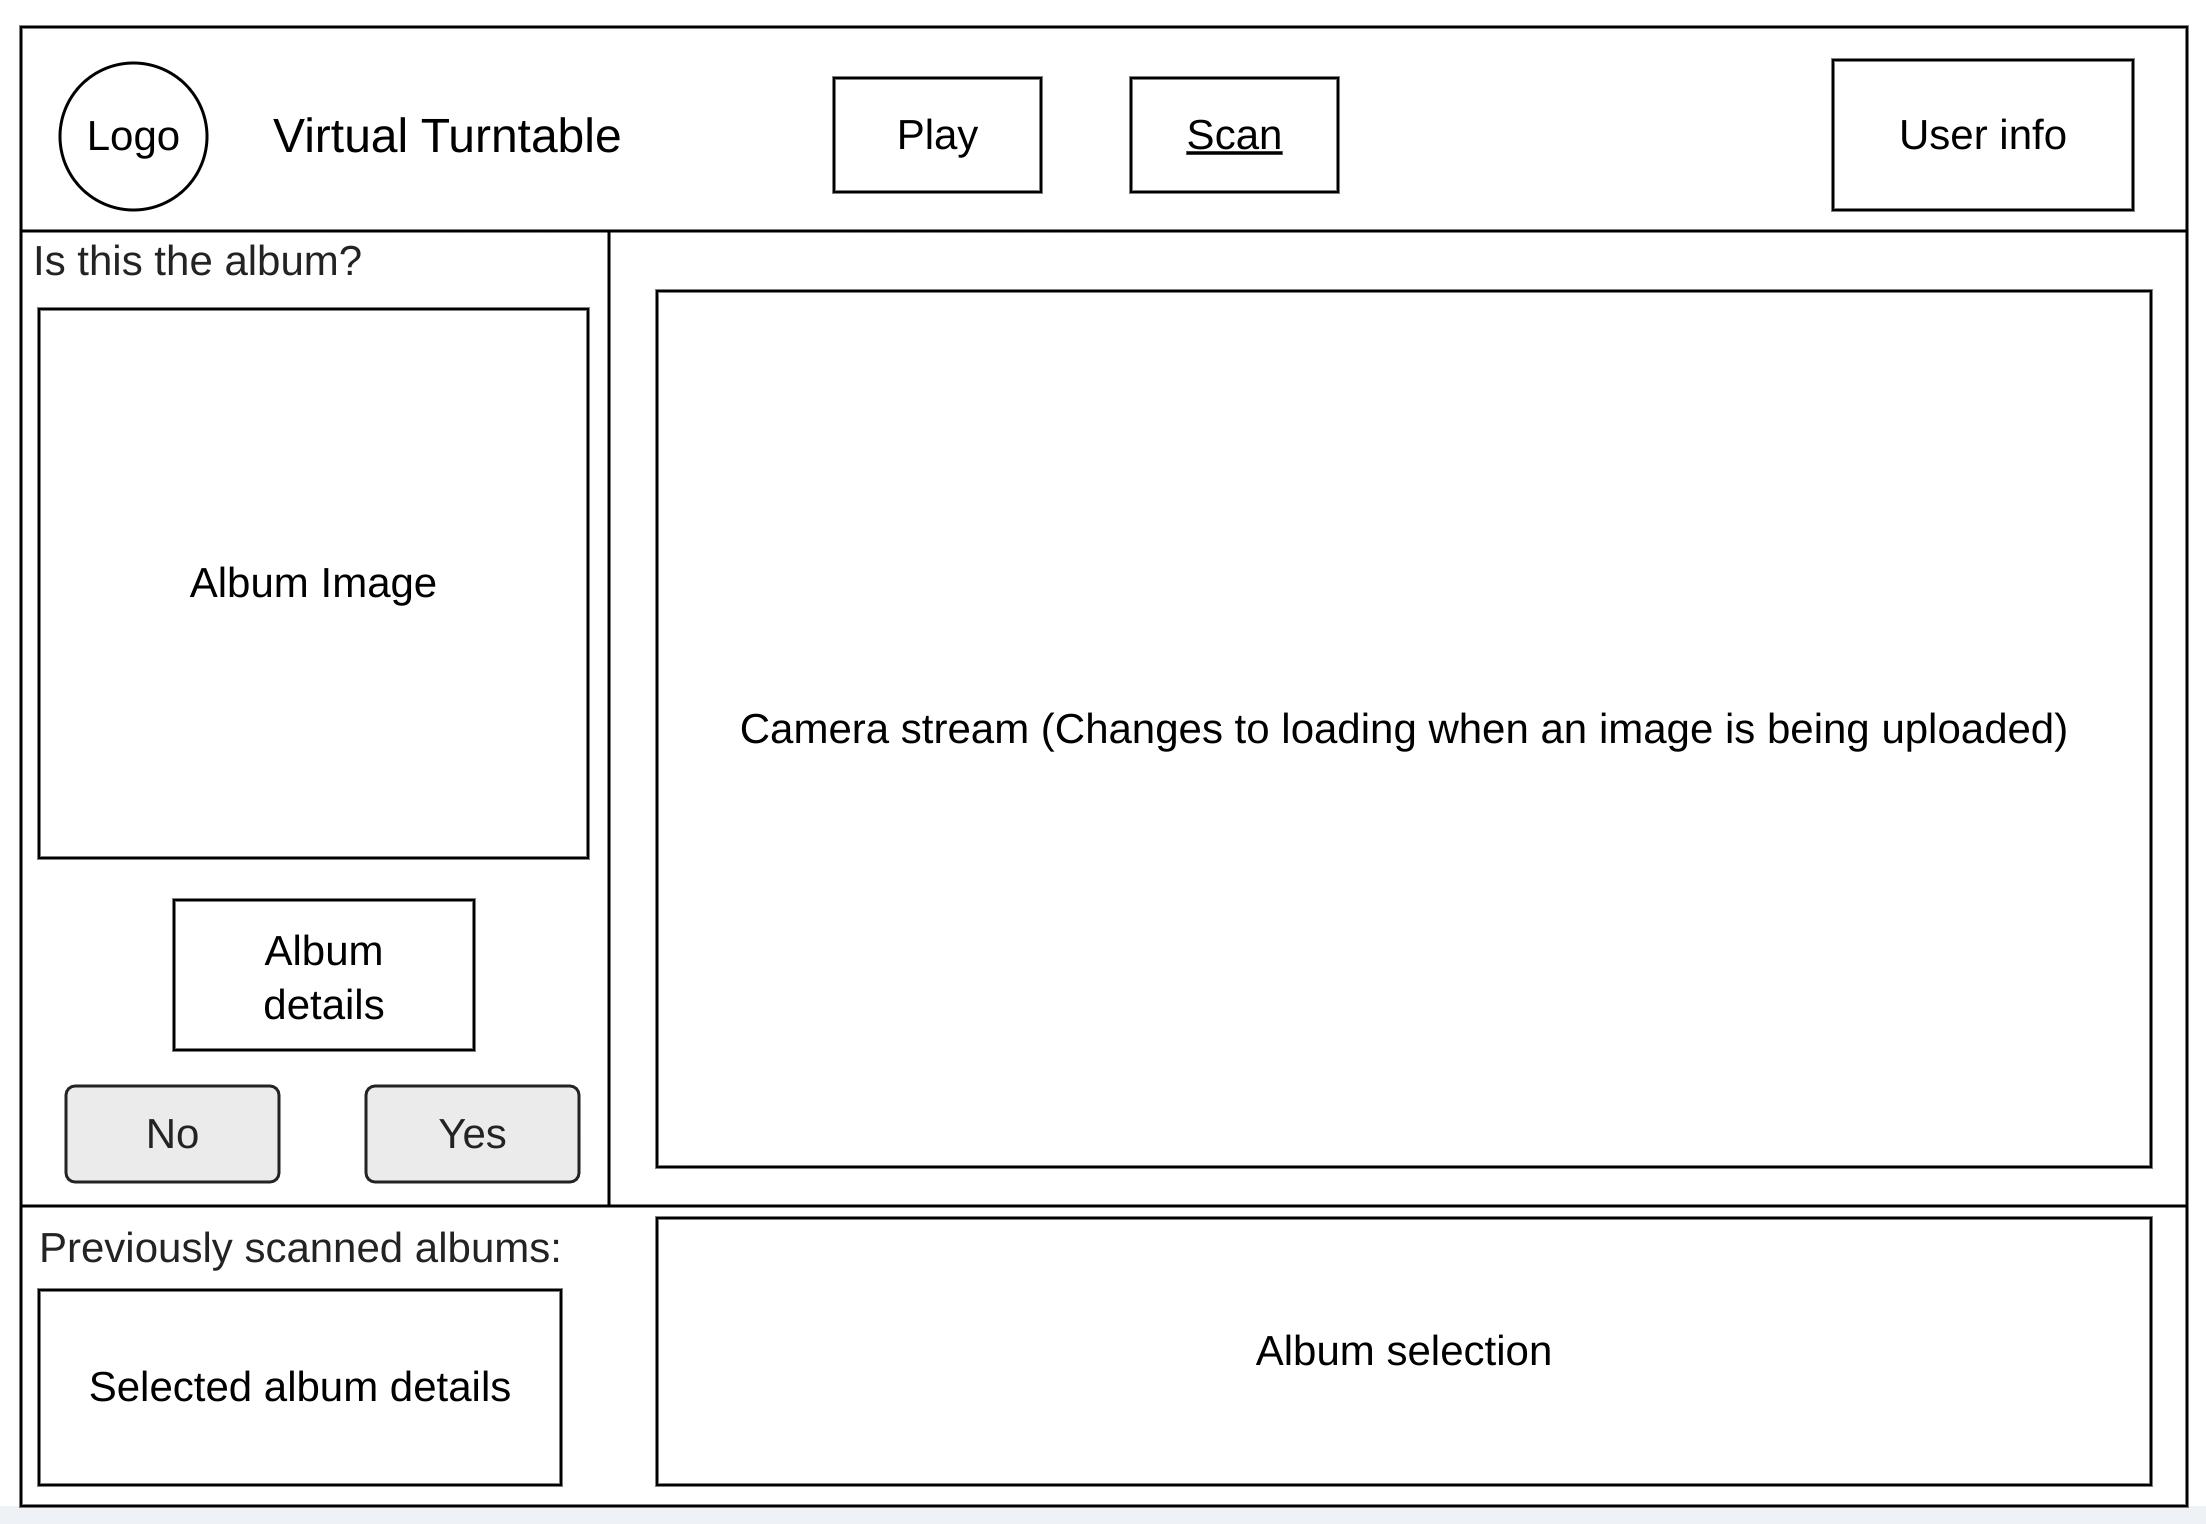
\includegraphics[width=0.6\linewidth]{figures/scan_screen_mockup.png}
    \caption{The scanning screen wireframe mockup}
    \label{fig:scan_screen_mockup}
\end{figure}


\subsubsection{Social Screen}
Figure~\ref{fig:social_screen_mockup} shows the social screen, where users can view collections belonging to others, either shared directly with them or made public. Users could use this page to see what their friends are listening to or discover new music.

\begin{figure} [H]
    \centering
    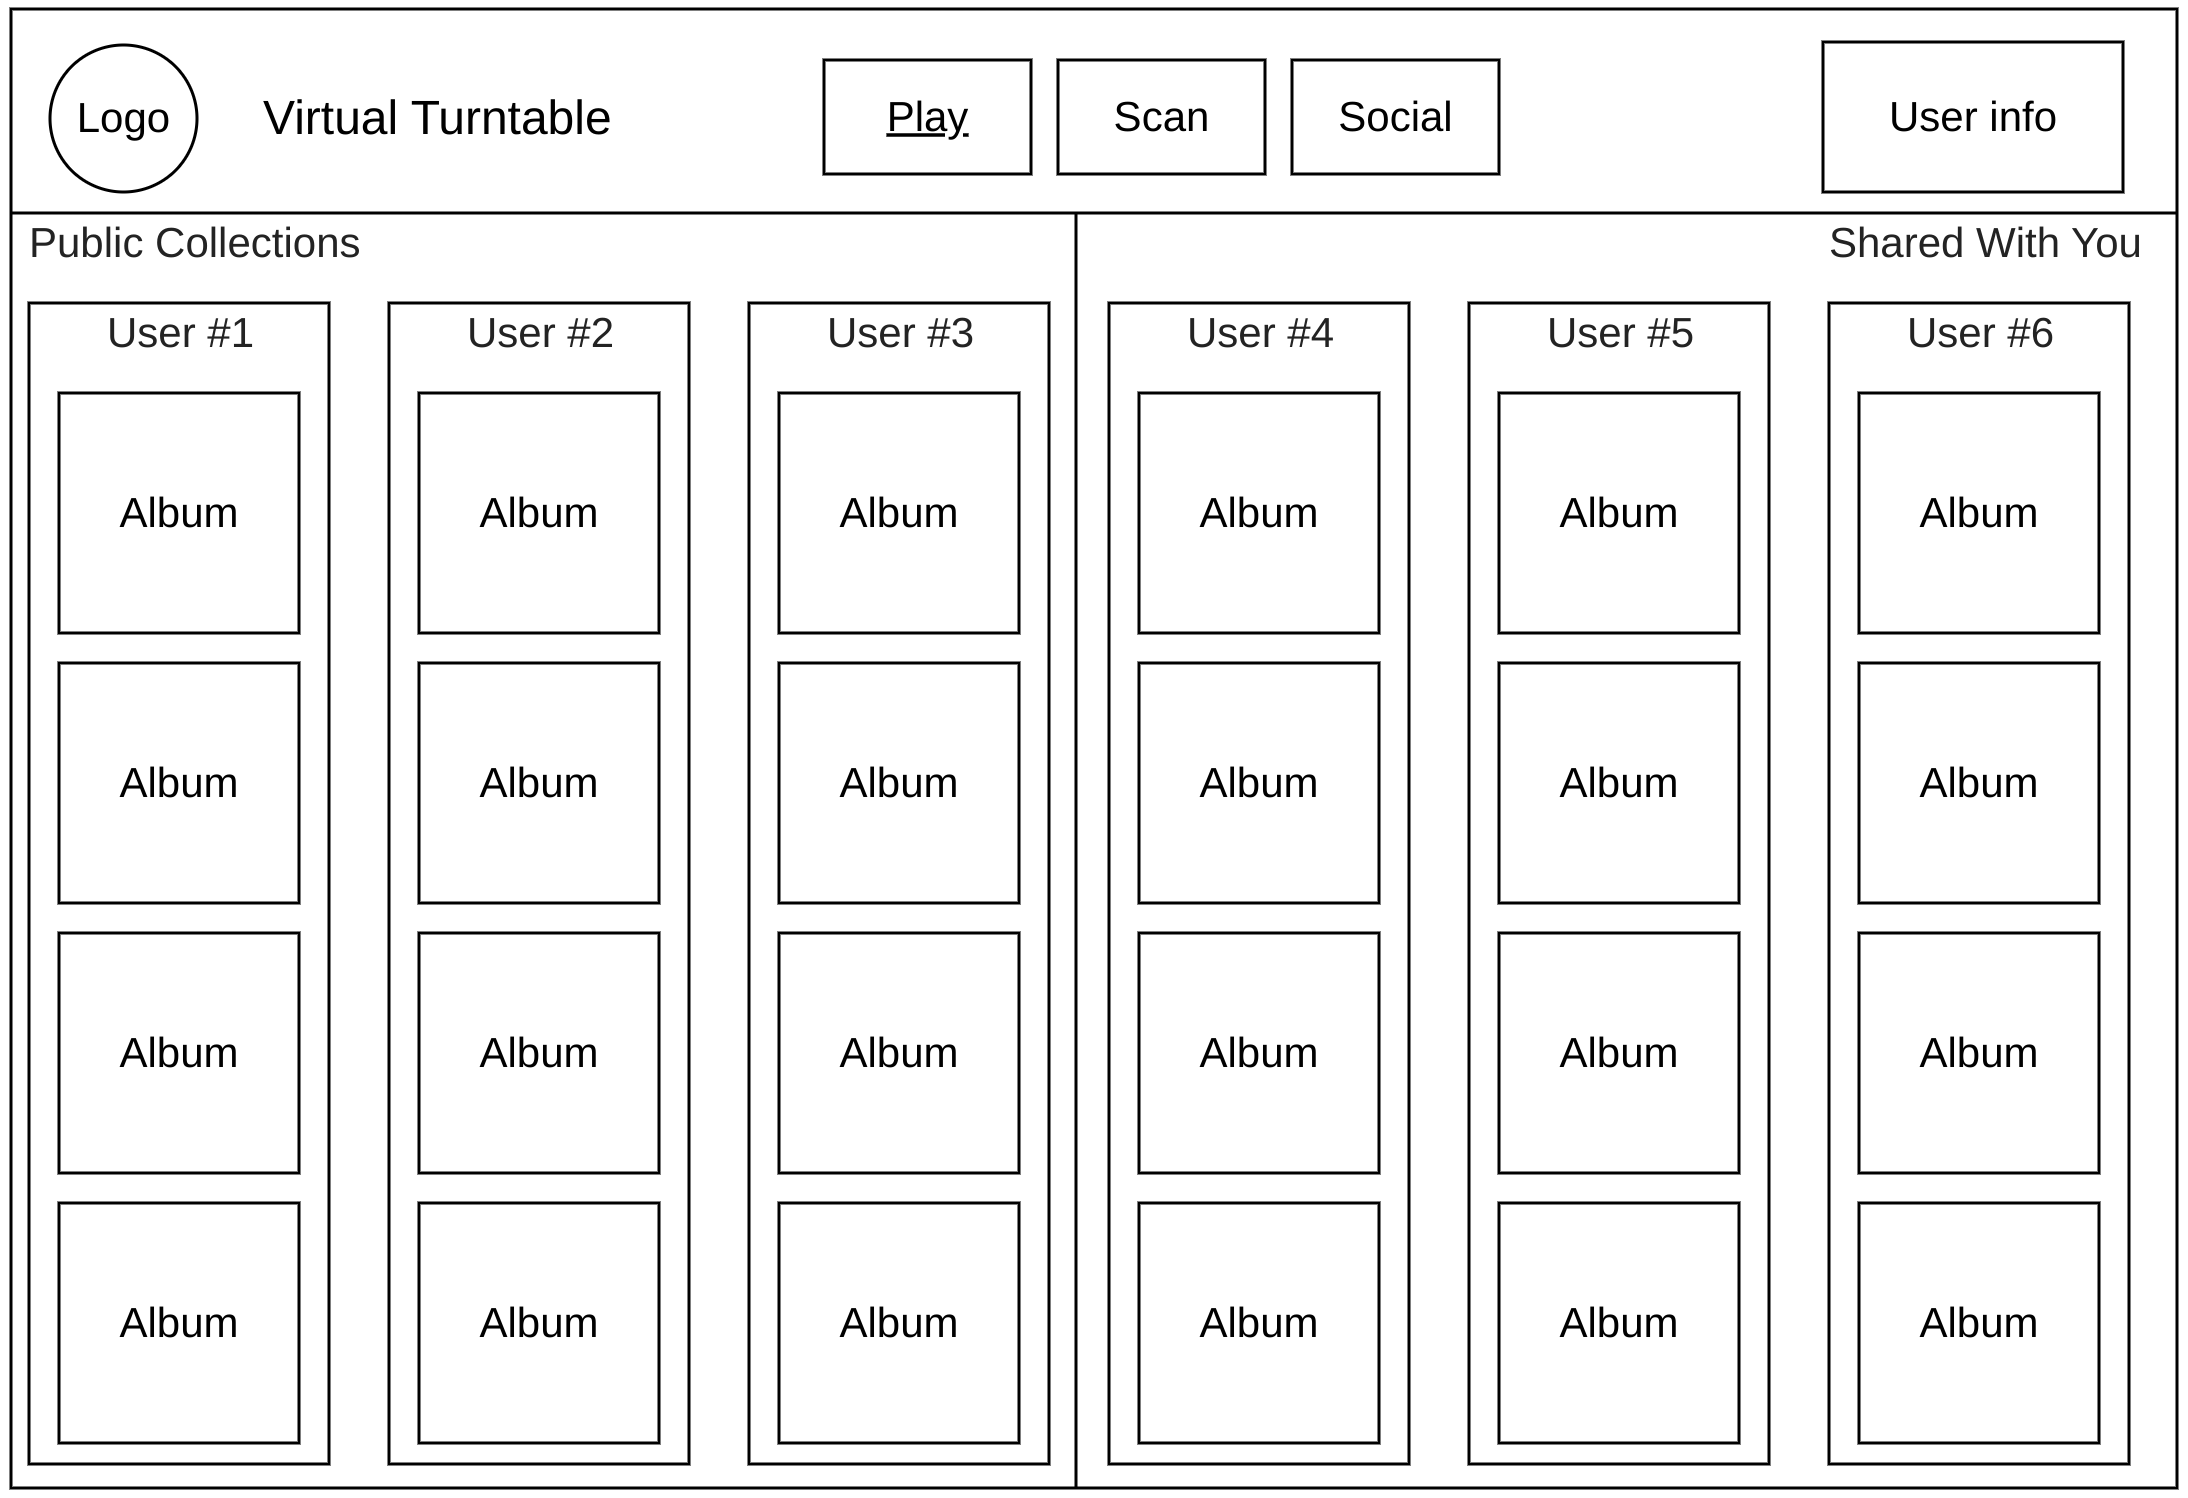
\includegraphics[width=0.6\linewidth]{figures/social_screen_mockup.png}
    \caption{The social screen wireframe mockup}
    \label{fig:social_screen_mockup}
\end{figure}

\section{Backend}~\label{sec:backend-design}
The project's backend was responsible for handling all business logic and data. It would mostly respond to API calls from the frontend except in cases where the backend needed to asynchronously push data to the frontend. That functionality would be achieved using WebSockets, which support bidirectional communication between the frontend and backend.

\subsection{Microservices split}
Since a microservices approach was adopted, the backend operations were divided into multiple services. As is discussed in Section~\ref{fig:final-arch}, it was decided to use a BFF (Backend for Frontend) pattern for one of these services. The remaining functionality was split into two services; one service handles the conversion of user-uploaded images into album data, while another manages all user-related data storage. The services could have been split further~\cite{7030212}, but this size was appropriate for the project's scope.

\subsubsection{BFF Service}
The BFF acts as a middleman between the frontend and various backend services, sometimes mirroring the endpoints of the other backend services. Its primary responsibility is to tailor the data returned to the frontend~\cite{BFF}. However, as this project is focused solely on a desktop web application, the pattern's potential to tailor data for different platforms was not fully utilised. If the application were later expanded to include additional platforms, the BFF could selectively limit data returned to given devices if it did not require it.

The BFF also handles the WebSocket connections to the frontend, allowing the backend to push data to the frontend when necessary. The main purpose of this functionality was to notify users on the front end when they received a request for a collection to be shared with them.

\subsubsection{Image to Album Service}
This service was the smallest of the three, encapsulating a particular functionality. Its intended design included endpoints responsible for identifying albums from various inputs, such as images of the album. This approach would allow different methods, such as OCR or reverse image search, to be handled through separate endpoints, with the caller choosing which to use. The service also hosted a way to search for albums using Spotify's API, which acted as a method to return an exact album from a guess that might have been generated by an identification method.

The separation of this functionality from the rest of the application's services means the application can handle a partial failure~\cite{7333476}. If this service were to fail, the rest of the application could still function, albeit without the ability to identify albums from images.

\subsubsection{User Data Service}
The user data service handled all tasks related to user data, such as storing and sharing collections. To maintain non-volatile storage, it would interact with a database detailed in Section~\ref{sec:database}. Each endpoint would perform a read or some edit of the data in the database, such as creating a user or sharing a collection.

\subsection{Database}~\label{sec:database}
This application could have been implemented as a stateless application, meaning there could be no capability to persist data across sessions. However, such an approach would limit functionality as there could be no personalisation for individual users. Since a Spotify account was already required for music playback, linking user data to that account became a logical next step, enabling data persistence across sessions.

\subsubsection{SQL vs NoSQL}
SQL databases are widely used in enterprise environments due to their reliability and consistency. However, relational databases are not necessarily optimal for web applications that require high scalability and availability~\cite{GANESHCHANDRA201513}. In contrast, NoSQL databases are designed with scalability and availability in mind~\cite{NoSQL}, often making them more suitable for such applications.
Although a NoSQL database like MongoDB would have been a good choice for this project, an SQL database was selected for its easy integration with FastAPI and SQLAlchemy, meaning quicker development and cleaner code, despite not being the most inherently scalable option. Though it should be noted that cloud database providers will often automatically scale the database as needed at a cost~\cite{CloudSQLScaling}.

\subsubsection{Diagram}
\begin{figure} [H]
    \centering
    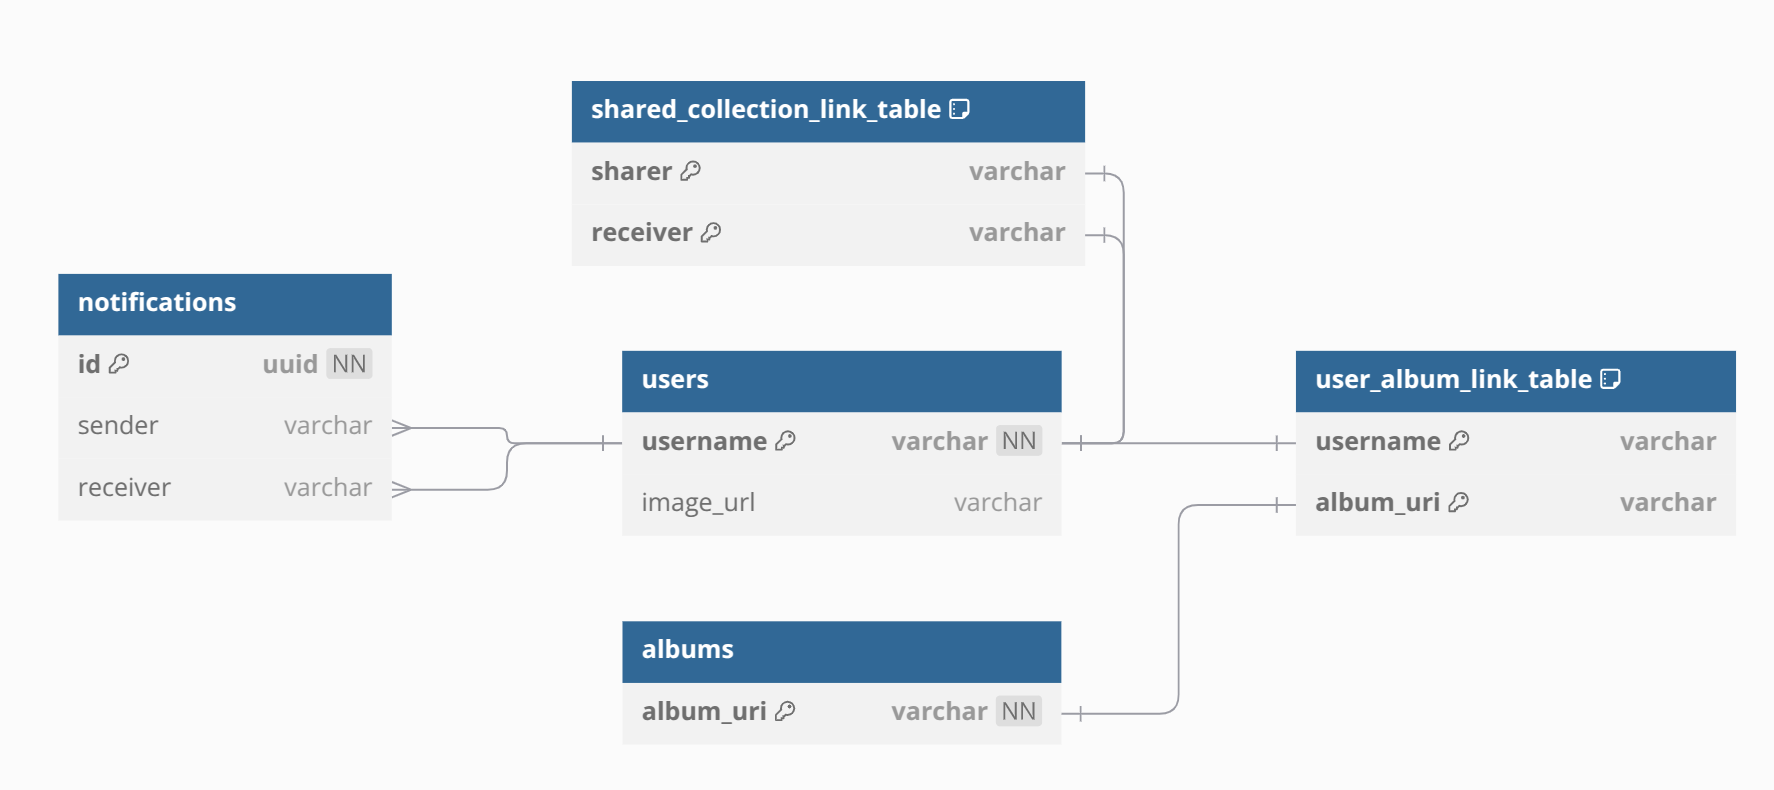
\includegraphics[width=0.6\linewidth]{figures/db_diagram.png}
    \caption{A diagram of the database using crow's foot notation}
    \label{fig:database-diagram}
\end{figure}

The database, shown in Figure~\ref{fig:database-diagram}, was designed in third normal form as this addresses insertion, deletion and update anomalies, ensuring data integrity. It meets first normal form as all data is atomic, second normal form as all non-key attributes are fully functionally dependent on the primary key, and third normal form as there are no transitive dependencies for non-key attributes~\cite{10.1145/320493.320489}.

Users are stored with their Spotify usernames as primary keys as Spotify guarantees unique usernames, allowing data in other tables to be linked through each user's username. Collections are represented with a link table that captures the many-to-many relationship between users and albums. A similar link table structure is used to manage the sharing of collections, tracking which users have shared access with each user. In addition, notifications regarding newly shared collections are stored in a separate table. These have to be stored between sessions as not all users are logged in simultaneously, so upon login, the user's notifications are fetched and displayed.

\subsubsection{DBMS Choice}
Since the choice was made to use a relational database, a specific database management system had to be selected. Since SQLAlchemy abstracts many of the differences among various DBMSs, they can easily be swapped out for another with no code changes, so the choice could be made solely based on the DMBSs' characteristics. The only notable exception is that SQLite does not enforce foreign key constraints by default, requiring manual enablement~\cite{SQLiteForeignKeys}.

Originally, SQLite was chosen because, as a file-based database, it could be easily stored within the Docker container running the user data service, simplifying deployment by reducing the number of containers. However, as the project grew, the need for concurrent database access became apparent, which SQLite does not support. Because of this, the decision was made to switch to either MySQL or PostgreSQL, both of which support concurrent access. For this project, the differences between these two systems were minor. PostgreSQL was selected since it is open-source, reducing the risk of future support being dropped.

\subsection{Security}
Security is an important consideration for any web application since functionality and access to user data are exposed to the internet~\cite{7980348}. Although the stored user data in this project is not particularly sensitive, it should still be safeguarded. To ensure this, measures had to be implemented for each backend service.

\paragraph{BFF} The BFF represents the most significant potential security risk, as it is the only service directly interacting with the frontend and, therefore, exposed to the public internet. To mitigate this risk, the BFF used authentication to verify requests to all endpoints related to user data. The exact details of this implementation are specified in Section~\ref{sec:backend-security}.

\paragraph{Image-to-Album \& User Data Services} These services operate behind the BFF and only need to accept requests from that single, predictable source. Because of this, they are designed to reject any requests originating from external sources, ensuring that only valid requests are processed.

\section{Testing}~\label{sec:test-design}
Defining the tests and success criteria before development was important to ensure the project was built to meet these objectives rather than retrofitting tests to match the final product. For most of the criteria listed in Section~\ref{sec:objectives}, it was necessary to establish tangible measurements to determine whether those criteria had been met.

\subsection{Primary Features}
For the two discussed primary features, these tests were defined:
\begin{itemize}
    \item The application should correctly identify albums with at least $95\%$ accuracy. This functionality must be accurate, but the threshold of $95\%$ is an arbitrary value chosen as the system is expected to reach a high but not perfect level of accuracy.
    \begin{description}
        \item[Verification:] Take a set of input images, modified to be poor and good quality, and calculate the system's accuracy. As the application will likely rely on external APIs, it is important that this functionality and the accuracies of any APIs are considered.
    \end{description}
    \item The application should play an album from start to finish without interruption.
    \begin{description}
        \item[Verification:] Play a set of albums on the application and verify that all play without interruption.
    \end{description}
\end{itemize}

\subsection{User Interface}~\label{sec:ui-tests}
Criteria relating to the user interface are harder to objectively assess as the quality of the interface is subjective. To determine if the objectives were met, a sample of users would need to be asked to use the application and provide feedback on the interface. This feedback could then be used to determine if the interface was easy to use and visually appealing and if users liked the saving and sharing features and found them useful.

For this purpose, the following survey was put together consisting of seven questions:
\begin{itemize}
    \item How easy was the application to use? ($1$ - $10$)
    \item How visually appealing was the application? ($1$ - $10$)
    \item How useful did you find the ability to save albums to your collection? ($1$ - $10$)
    \item How valuable did/would you find the social features? ($1$ - $10$)
    \item Any extra comments? (Free text)
\end{itemize}

These questions cover the main objectives of the user interface and should, therefore, provide a good indication of whether the objectives were met.

\subsection{Code Quality}
The last set of criteria, relating to good software development practices, are generally more objective and, as such, are more easily verifiable. For this, the following tests were defined:
\begin{itemize}
    \item The codebase should maintain at least $95\%$ test coverage. This threshold is high enough to guarantee that much of the code is tested, but it is not so high that it becomes difficult to maintain.
    \begin{description}
        \item[Verification:] Run all test suites and verify the line coverage and branch coverage exceeds $95\%.$
    \end{description}
    \item All tests must pass successfully.
    \begin{description}
        \item[Verification:] Run all test suites and verify that all tests pass.
    \end{description}
    \item Code should be evaluated by linters and formatters to maintain consistency and quality.
    \begin{description}
        \item[Verification:] For Python code, run Ruff for formatting and Pylint for linting. For Typescript, run Biome for both formatting and linting. Both should pass without errors.
    \end{description}
    \item A continuous deployment system should automatically redeploy the application following any code change.
    \begin{description}
        \item[Verification:] Push a change to the repository and verify that the application is redeployed with the change in place.
    \end{description}
    \item An automated system should be in place to update dependencies.
    \begin{description}
        \item[Verification:] An automated tool for dependency management should be configured on the repository to run at a given interval.
    \end{description}
\end{itemize}

Most of these criteria can be met using tools such as GitHub Actions, which can run tests on each commit and trigger application deployments. Dependabot can scan and update the repository’s dependencies as new releases become available. Additionally, linters and formatters can be executed as pre-commit hooks, preventing code below a defined quality threshold from being committed to the repository.

A side effect of having high test coverage is a reduced risk associated with dependency updates since tests help verify that the update has not broken any functionality.
